


%%%%%%%%%%%%%%%%%%%%%%%%%%%%%%%%%%%%%%%%%%%%%%%%%%%%%%%%%%%%%%%%%%%%%%%%
\section{Agentes Racionais}


\begin{frame}

\begin{center}
{\huge Capítulo 2 -- Agentes Racionais}
\end{center}

\end{frame}




%--------------------------------------------
\begin{frame} %[allowframebreaks=0.9]

    \frametitle{O que é um Agente?}

\begin{block}{Qualquer entidade (humana ou artificial) que:}
  
  \begin{itemize}
    \item está \textbf{imersa} ou \textbf{situada} em um ambiente (físico, virtual/simulado) 
    \item \textbf{percebe} ou \textbf{sente} seu ambiente através de sensores (ex. câmeras, microfone, teclado, finger, ...)
    \item \textbf{age} sobre ele através de atuadores (ex. vídeo, auto-falante, impressora, braços, ftp, ...)
    \item \textbf{possui objetivos} próprios:
explícitos ou implícitos
    \item \textbf{escolhe} suas ações em função das suas percepções para atingir seus objetivos
  
  \end{itemize}
  
\end{block}

\end{frame}
%--------------------------------------------


%--------------------------------------------
\begin{frame} %[allowframebreaks=0.9]

    \frametitle{Agente Situado x Não-Situado}

    
\begin{figure}[!ht]
\centering
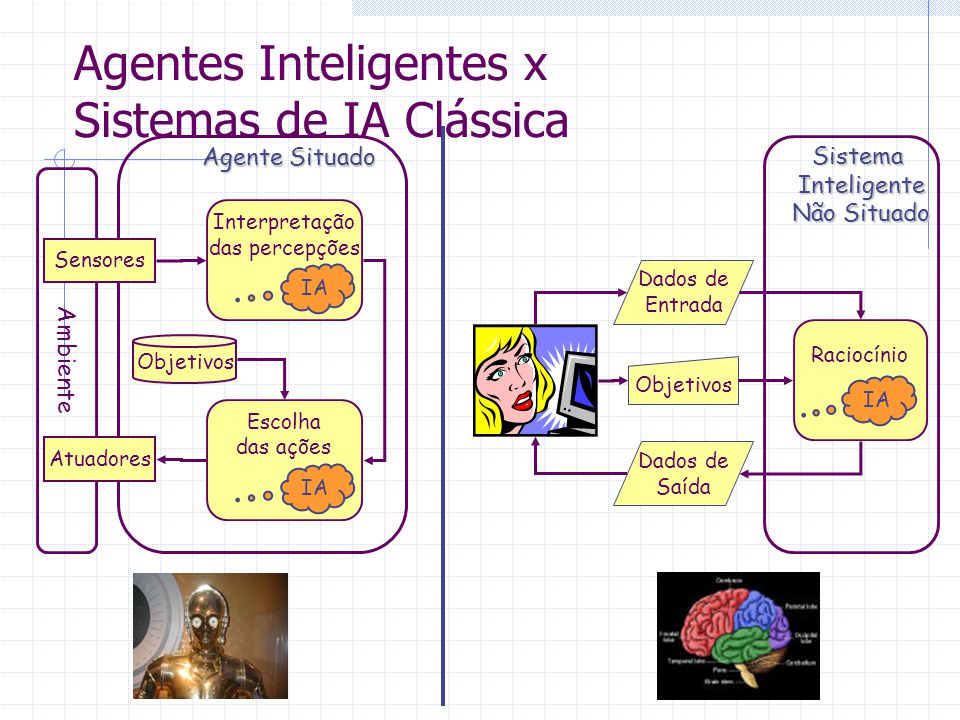
\includegraphics[height =.65\textheight,width=.8\textwidth]{figuras/agente_situado.jpg}
\caption{Agente situado versus a visão clássica de sistemas inteligentes}
%\label{ag_01}
\end{figure}

\end{frame}
%--------------------------------------------


%--------------------------------------------
\begin{frame} %%%[allowframebreaks=0.9]

    \frametitle{O que é um Agente Racional?}

\begin{block}{}
  
 \begin{itemize}
      \item Agente Racional 
 \begin{itemize}
        \item faz a melhor ação possível dado um conjunto de percepções
        \item segue o princípio da racionalidade:\\ 
dada uma seqüência perceptiva, o agente escolhe, segundo seus conhecimentos, 
as ações que melhor satisfazem seu objetivo
      \end{itemize}

\begin{itemize}
  \item Limitações de:\\
  sensores\\
  atuadores\\
  raciocinador (conhecimento, tempo, etc.)
\end{itemize}

    \end{itemize}
  
\end{block}

\end{frame}
%--------------------------------------------



%--------------------------------------------
\begin{frame} [allowframebreaks=0.9]

    \frametitle{Outras propriedades freqüentemente associadas aos Agentes}

 
    \begin{itemize}
      \item Autonomia:\\
raciocínio, comportamento guiado por objetivos ou \\
\textit{reatividade}

\begin{itemize}
  \item Requer máquina de inferência e base de conhecimento
  \item Essencial em sistemas especialistas, controle, robótica, jogos, agentes na internet ...
\end{itemize}
      
    \item Adaptabilidade \& aprendizagem
             
    \begin{itemize}
             
    \item Capacidade de adaptação a situações novas, para as quais não foi fornecido todo o      conhecimento necessário com antecedência 

     \item Duas implementações: sistema com  
           aprendizagem 
           e/ou programação declarativa
  
     \item Essencial em agentes na internet, interfaces amigáveis ...
   
    \end{itemize}
             
             
    \item Comunicação \& Cooperação (sociabilidade)
         \begin{itemize}
          \item  Protocolos padrões de comunicação, cooperação, negociação
          \item  Raciocínio autônomo sobre crenças e confiabilidade
          \item  Arquiteturas de interação social entre agentes
                      
         \end{itemize}
         
                
    \item Personalidade
    
    \begin{itemize}
      \item IA + modelagem de atitudes e emoções (computação afetiva)
      \item Essencial em entretenimento digital, realidade virtual, interfaces amigáveis ... 
    \end{itemize}
    
    \item Continuidade temporal (persistência)
    \begin{itemize}
      \item Requer interface com sistema operacional e banco de dados
    \item Essencial em filtragem, monitoramento, controle, ...
    \end{itemize}
    
    
 \item Mobilidade (caso internet)
  \begin{itemize}
     \item Requer itens como:
     \begin{enumerate}
       \item Interface com rede
       \item Protocolos de segurança
       \item Suporte a código móvel
     \end{enumerate}

    \item Essencial em agentes de exploração da internet, ...
         
     \end{itemize}      
                  
    \end{itemize}
 
\end{frame}
%--------------------------------------------

%--------------------------------------------
\begin{frame} %[allowframebreaks=0.9]

 \frametitle{Exercício}
    
\begin{figure}[!ht]
\centering
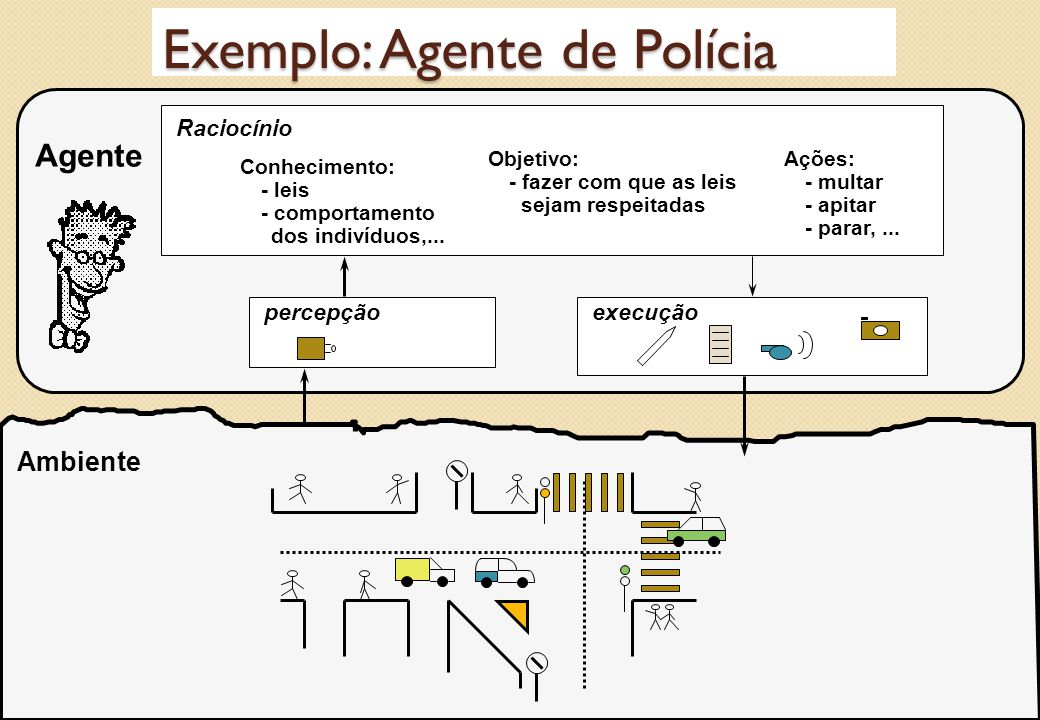
\includegraphics[height =.6\textheight,width=.8\textwidth]{figuras/agente_policial.jpg}
\caption{Exercício: enumere as características citadas a este exemplo -- ao final do capítulo este exercício deve ser rediscutido}
\label{agente_policial}
\end{figure}

\end{frame}
%--------------------------------------------



\subsection{Tipos de Agentes}
\begin{frame} [allowframebreaks=0.9]
\frametitle{Tipos de Agentes}

Em geral os agentes encontram-se em  dois grupos (2 classes):

\begin{description}

 \item[Agentes Reflexivos:] geralmente são agentes simples, escolhem suas 
 ações baseados \textbf{exclusivamente} nas percepções que têm do ambiente. 
 Normalmente possuem uma representação do conhecimento implícita  no código, por não  possuirem  memória, não tem histórico dos fatos  e das ações que executou.
 
 \begin{itemize}
   \item Nota: nestes slides, ora são chamados de  \textit{reativos}
   
   \item Na 3a. versão do livro do Russel e Norvig -- utiliza-se o termo \textit{reflexivo}
   
   \item Ver fundamentação biológica para este termo -- está correta
   
   \item Nos primórdios da área: o termo é \textit{reativo} 
   
 \end{itemize}

 
\newpage

  \item[Agentes Cognitivos:]  têm uma representação simbólica explícita do seu ambiente, no qual eles podem argumentar e predizer eventos futuros. Estes são dirigidos por intenções, isto é, por metas explícitas que conduzem seu comportamento e os tornam capazes de escolher entre possíveis ações. 
  Engloba as características: \textit{\textcolor{blue}{percepção, ação, comunicação,  representação, 
  motivação, deliberação, raciocínio e aprendizagem}}. 

\end{description}

\end{frame}
%--------------------------------------------------------------------------
\begin{frame}

  \frametitle{Arquitetura clássica de um agente reflexivo}
    
\begin{figure}[!ht]
\centering
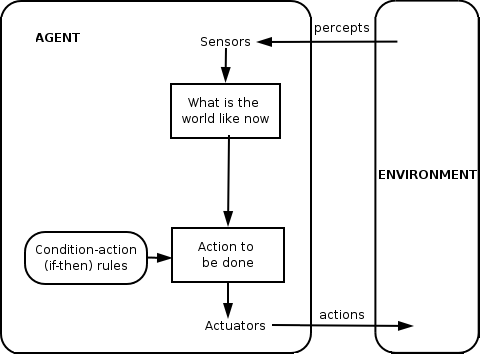
\includegraphics[width=.6\textwidth]{figuras/agente_reflexivo.png}
\caption{Arquitetura clássica -- reflexivo}
\label{ag_01}
\end{figure}
    
\end{frame}

%--------------------------------------------------------------------------
\begin{frame}

  \frametitle{Arquitetura clássica de um agente cognitivo (\textit{que aprende algo!}}
    
\begin{figure}[!ht]
\centering
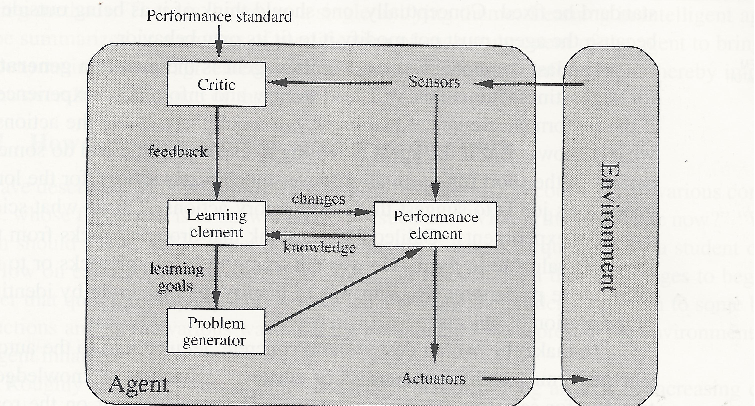
\includegraphics[height =.6\textheight,width=.7\textwidth]{figuras/agente_aprendizagem.pdf}
\caption{Arquitetura clássica -- agente cognitivo com aprendizagem}
\label{ag_02}
\end{figure}
    
\end{frame}



%--------------------------------------------
\subsection{Arquiteturas de Agentes}
\begin{frame} %[allowframebreaks=0.9]

\frametitle{Arquiteturas ou Modelos de Agentes}

\begin{block}{Destes 2 grupos(reflexivo e cognitivo), delinea-se algumas arquiteturas:}
  
    \begin{itemize}
      \item Agente tabela (menos complexo -- mais baixo-nível $\downarrow $)
      \item Agente reativo
      \item Agente reativo com estado interno 
      \item Agente baseado em objetivos (com \textit{alguma} cognição)
      \item Agente otimizador
      \item Agente adaptativo (mais complexo -- mais alto-nível $\uparrow $)
    \end{itemize}
  
\end{block}

\end{frame}
%--------------------------------------------


%--------------------------------------------

\begin{frame} %[allowframebreaks=0.9]

    \frametitle{Genericamente todos seguem algo como:}

Um agente pode ser visto como um \textcolor{red}{\texttt{mapeamento}}: 
\textbf{seqüência e/ou fusão de percepções $\Rightarrow$  ação}

\begin{figure}[!ht]
  \centering
  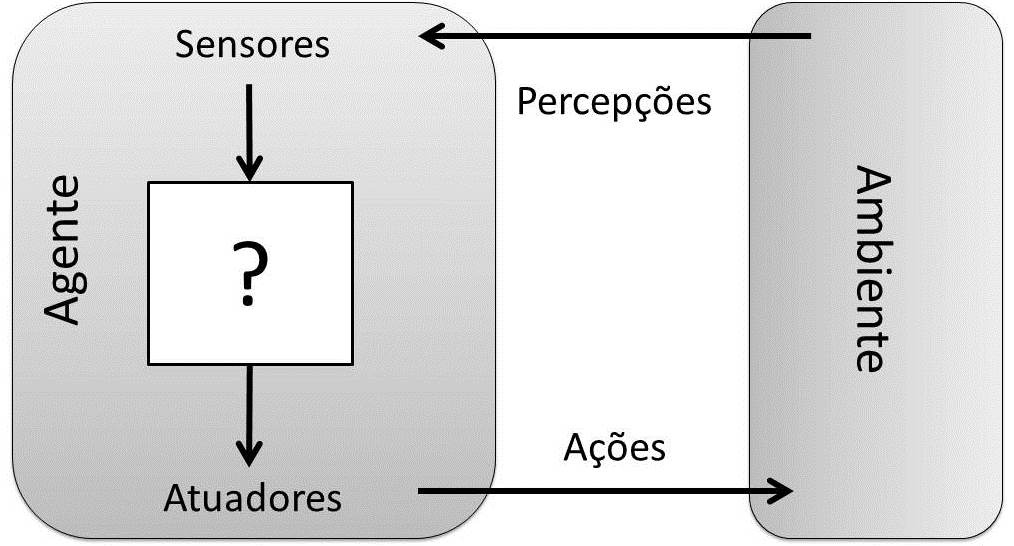
\includegraphics[height =.5\textheight,width=.7\textwidth]{figuras/agente_generico.jpg}
  \caption{Agente Genérico}
%\label{ag_01}
\end{figure}
%--------------------------------------------
\end{frame}

%--------------------------------------------

\begin{frame} %[allowframebreaks=0.9]

    \frametitle{Agente Tabela – é mesmo um agente racional?}

\begin{figure}[!ht]
  \centering
  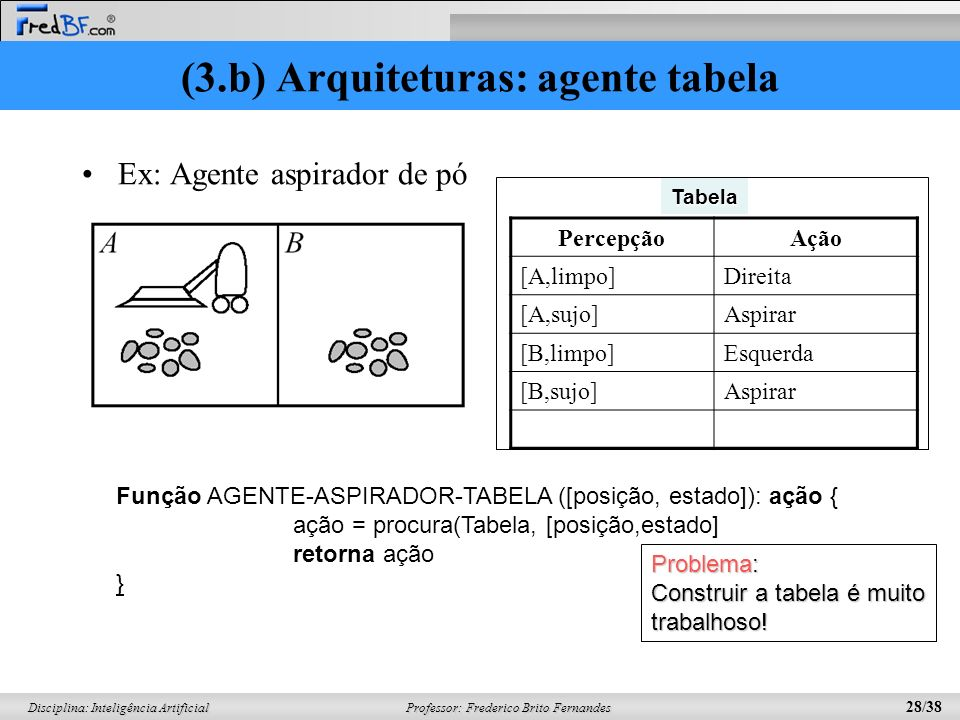
\includegraphics[height =.6\textheight,width=.7\textwidth]{figuras/agente_tabela.jpg}
  \caption{Agente Tabela -- seguem os \textit{copyrights}}
%\label{ag_01}
\end{figure}

\end{frame}
%--------------------------------------------



%--------------------------------------------

\begin{frame} %[allowframebreaks=0.9]

    \frametitle{Agente Tabela}

\begin{itemize}
  \item Limitações
  \begin{itemize}
    \item Mesmo problemas simples requerem tabelas muito grandes 
Ex. jogo de xadrez $30^{100}$
    \item Nem sempre é possível, por ignorância ou questão de tempo, construir a tabela 
    \item  Não há autonomia nem flexibilidade
    
    \item Este \textit{infeliz} entra em pane se o conhecimento  não estiver descrito na tabela (inferior há uma regra \textit{if-then})
    
  \end{itemize}
  
  \item Ambiente
\begin{itemize}
  \item do tipo acessível:  determinista, episódico, 
   estático, discreto e minúsculo!
   
\end{itemize}
  
\end{itemize}
\end{frame}
%--------------------------------------------



\begin{frame} %[allowframebreaks=0.9]

\frametitle{Agente Reativo}

\begin{figure}[!ht]
  \centering
  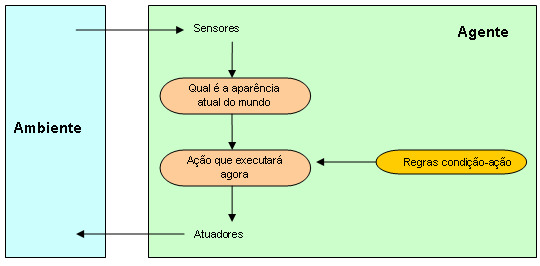
\includegraphics[height =.6\textheight,width=.7\textwidth]
  {figuras/agente_reativo.jpg}
  \caption{Agente Reativo -- seguem os \textit{copyrights}}
%\label{ag_01}
\end{figure}

\end{frame}
%--------------------------------------------



%--------------------------------------------

\begin{frame} %[allowframebreaks=0.9]

    \frametitle{Agente Reativo}

\begin{itemize}
  \item Vantagens e desvantagens
  \begin{itemize}
    \item Regras condição-ação: representação inteligível, modular e eficiente\\ 
Ex: \texttt{Se velocidade $>$ 60 então multar}
   \item Não pode armazenar uma seqüência perceptiva, pouca autonomia
  \end{itemize}
  
  \item Ambientes
\begin{itemize}
  \item Reflexo imprescindível em ambientes dinâmicos 
  \item Acessível, episódico, pequeno 
\end{itemize}
  
\end{itemize}
\end{frame}
%--------------------------------------------


\begin{frame} %[allowframebreaks=0.9]

 \frametitle{Agente reativo com estado interno}

\begin{figure}[!ht]
  \centering
  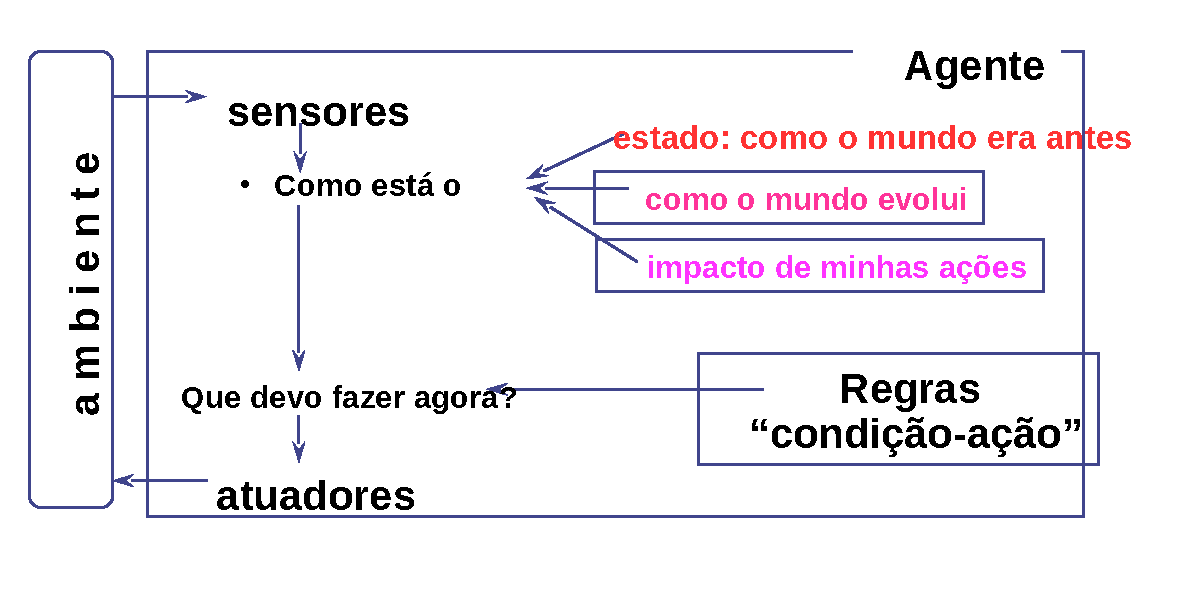
\includegraphics[height =.6\textheight,width=.7\textwidth]
  {figuras/agente_reativo_com_estado_interno.pdf}
  \caption{Agente reativo com estado interno -- seguem os \textit{copyrights}}
%\label{ag_01}
\end{figure}

\end{frame}
%--------------------------------------------



%--------------------------------------------

\begin{frame} %[allowframebreaks=0.9]

    \frametitle{Agente reativo com estado interno}

\begin{itemize}
  \item Desvantagens
  \begin{itemize}
    \item pouca autonomia

   \item não tem objetivo, não encadeia regras
   
   \item melhorar a figura .... \textit{como está o mundo agora?}
  \end{itemize}
  
  \item Ambientes
\begin{itemize}
  \item determinista e pequeno 
  \item Ex. Tamagotchi -- sucesso 
\end{itemize}
  
\end{itemize}
\end{frame}
%--------------------------------------------


\begin{frame} %[allowframebreaks=0.9]

 \frametitle{Agente baseado em objetivo}

\begin{figure}[!ht]
  \centering
  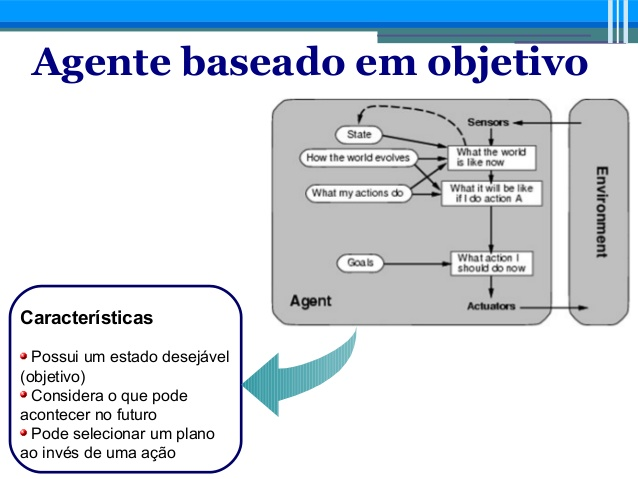
\includegraphics[height =.7\textheight,width=.7\textwidth]
  {figuras/agente_baseado_em_objetivo.jpg}
  \caption{Agente baseado (orientado) em objetivo -- seguem os \textit{copyrights}}
%\label{ag_01}
\end{figure}

\end{frame}
%--------------------------------------------



%--------------------------------------------

\begin{frame} %[allowframebreaks=0.9]

    \frametitle{Agente baseado em objetivo}

\begin{itemize}
  \item Vantagens e desvantagens

  \begin{itemize}
    \item Mais complicado e ineficiente,  porém mais flexível, autônomo
    \item Não trata objetivos conflitantes
  \end{itemize}
  
  \item Ambientes

\begin{itemize}
  \item determinista 
  \item Ex.ex.: xeque-mate no xadrez
\end{itemize}
  
\end{itemize}
\end{frame}
%--------------------------------------------

%--------------------------------------------


\begin{frame} %[allowframebreaks=0.9]

 \frametitle{Agente otimizador (\textit{utility based})}

\begin{figure}[!ht]
  \centering
  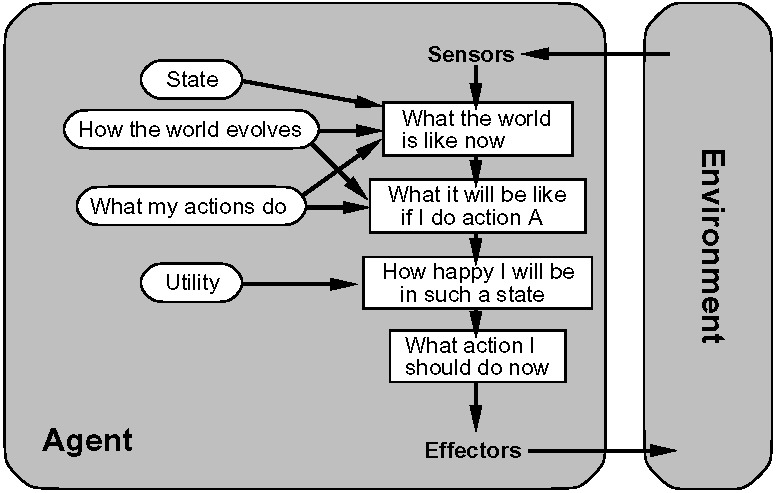
\includegraphics[height =.6\textheight,width=.7\textwidth]
  {figuras/agente_otimizador.jpg}
  \caption{Agente otimizador -- seguem os \textit{copyrights}}
%\label{ag_01}
\end{figure}

\end{frame}

%----------------------------------------------------------------------------------------

\begin{frame} %[allowframebreaks=0.9]

    \frametitle{Agente otimizador}

\begin{itemize}
  \item Ambiente: sem restrição
  
  \item Desvantagem: não  tem adaptabilidade
  
  \item Ex. \texttt{alguns} motoristas do Brasil\\
    Segurança e velocidade – conflito!
  
\end{itemize}
\end{frame}
%--------------------------------------------


%--------------------------------------------


\begin{frame} %[allowframebreaks=0.9]

 \frametitle{Agente que aprende (\textit{learning agent})}

\begin{figure}[!ht]
  \centering
  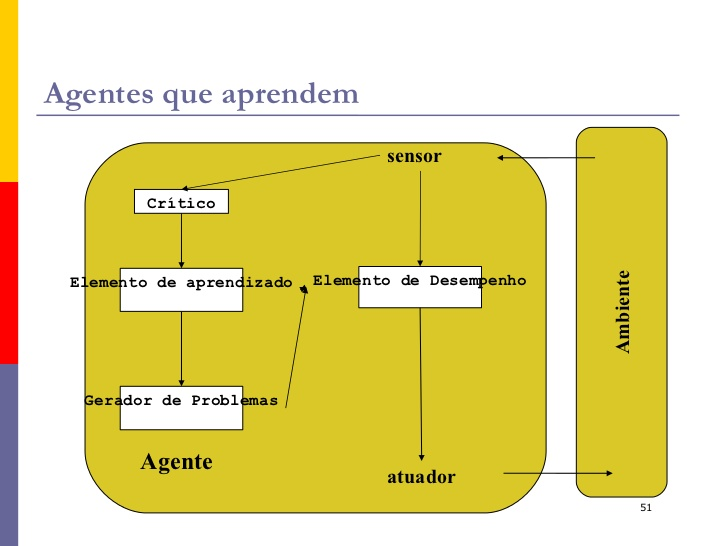
\includegraphics[height =.6\textheight,width=.7\textwidth]
  {figuras/agentes_que_aprendem.jpg}
  \caption{Agente que aprende -- seguem os \textit{copyrights}}
%\label{ag_01}
\end{figure}

\end{frame}
%--------------------------------------------



%--------------------------------------------

\begin{frame} %[allowframebreaks=0.9]

    \frametitle{Agente que aprende}

\begin{itemize}
  \item Ambiente: sem restrição
  
  \item Vantagem:  tem adaptabilidade (aprende)
  
  \item Ex.  motoristas em um GPS
  
\end{itemize}
\end{frame}
%--------------------------------------------



\section{Construindo de Agentes Racionais}

\begin{frame}%%[allowframebreaks=0.9]

% \frametitle{Uma medida de eficácia para estes agentes (racionais)?}
   \frametitle{Metodologia de desenvolvimento destes agentes racionais}
  \begin{block}{\textbf{PEAS} = Peformance, Ambiente (\textit{Enviroment}), Ação e Sensores}
  
   \begin{description}
  
     \item[Peformance:] como ter um indicativo de sucesso
     
    \item[Ambiente:]  cuidado deve ser sempre 
especificar o ambiente
          
   \item[Ação:] o que vai fazer?
                          
  \item[Sensores:] o que vai perceber?

  \item[Outros:] agentes da comunidade (falta isto na construção de agentes), ou seja um SMA!

          
   \end{description}
  \end{block}    
   
\end{frame}


%--------------------------------------------


\begin{frame} %[allowframebreaks=0.9]

 \frametitle{Exemplo ao avaliar (projetar ...) SMAs}

\begin{figure}[!ht]
  \centering
  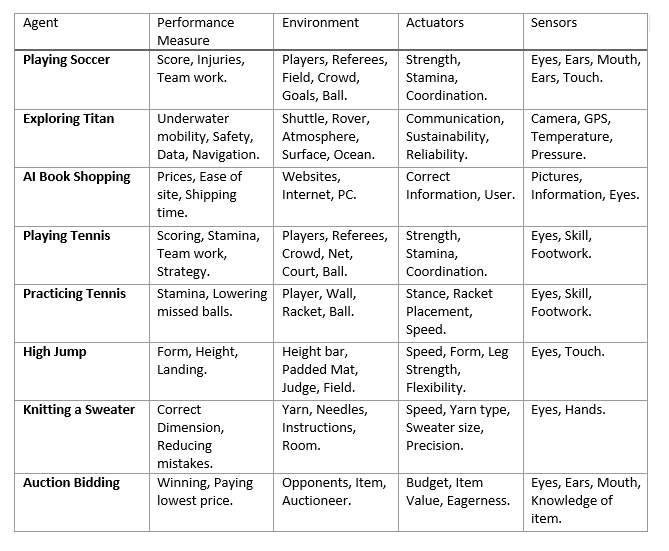
\includegraphics[height =.7\textheight,width=.8\textwidth]
  {figuras/PEAS01.png}
  \caption{Um bom exercício para reflexão -- seguem os \textit{copyrights}}
%\label{ag_01}
\end{figure}

\end{frame}
%--------------------------------------------

%--------------------------------------------

\begin{frame} %[allowframebreaks=0.9]

 \frametitle{Exemplo ao avaliar (projetar ...) SMAs}

\begin{figure}[!ht]
  \centering
  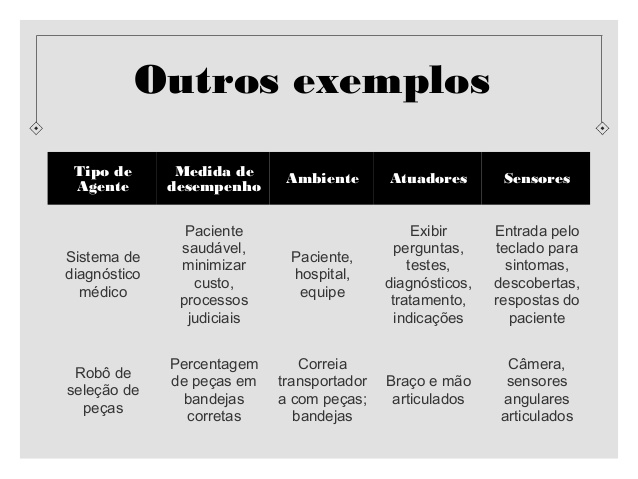
\includegraphics[height =.7\textheight,width=.8\textwidth]
  {figuras/PEAS02.jpg}
  \caption{Um bom exercício para reflexão -- seguem os \textit{copyrights}}
%\label{ag_01}
\end{figure}

\end{frame}

\begin{frame} %[allowframebreaks=0.9]

 \frametitle{Volte ao exemplo do agente policial -- ver figura \ref{agente_policial}}

\begin{itemize}
  \item Quem é seu ambiente?
  \item Quem são seus sensores?
    \item Quem são seus atuadores?
    \item Qual é o seu mecanismo de raciocínio?
    \item Há outros agentes?
    \item Como é o seu ambiente (discreto, episódico..... -- ver características do livro do Norvig--Russel)?
    \item Sua interação com o ambiente?
    \item Há outros agentes? Quais? Comunidades?
\end{itemize}


\end{frame}

%-----------------------------------------------------------

\begin{frame} %[allowframebreaks=0.9]

 \frametitle{Resumo do capítulo}

\begin{enumerate}
  \item Vocabulário
  \item Uma gama de agentes ...
    \begin{itemize}
    \item Dos reativos: os mais simples, e quando numa comunidade são todos iguais
    \item Aos cognitivos: os mais complexos, e quando numa comunidade apresentam
    uma metáfora social de humanos
  \end{itemize}
  
  \item Como iniciar um desenvolvimento de SMAs 
  
  \item Falta: porque soluções de SMAs são atrativas
    \item Falta: diferença de SMAs com RDPs
    \item Falta: Coordenação etc
        \item Falta: Planejamento etc
    
\end{enumerate}


\end{frame}
